\section{Requerimientos no funcionales}

\subsection{Mantenibilidad}

En \cite{measuring_maintainability}, los autores hicieron una valoración de las métricas utilizadas para evaluar la mantenibilidad del software, según el estandar ISO/IEC 9126, encontrando deficiencias en la métrica más usa, el Indice de Mantenibilidad, o MI por sus siglas en ingles. Encontradas las deficiencias en claridad, crearon nuevas métricas basados en las subcaracterísticas usadas para medir la mantenibilidad de un software. Las subcaracterísticas atadas a la Mantenibilidad según el estandar son:

\begin{itemize}
 \item \textbf{Analizabilidad (Analisability)}: Se refiere a la dificultad de saber en que parte del software se debe hacer un cambio y, a su vez, cuales tienen deficiencias.
 \item \textbf{Cambiabilidad (Changeability)}: Se refiere al nivel de dificultad para hacer adaptaciones al software.
 \item \textbf{Estabilidad (Stability)}: Compete a este el análisis de cuan estable es el software mientras este está sufriendo algún cambio
 \item \textbf{Probabilidad (Testability)}: Responde a la pregunta, ¿cuán difícil es probar el sistema luego de haberle hecho una modificación?
 \item \textbf{Conformidad de mantenibilidad (Mantenibility conformance)}: Éste se refiere al análisis del cumplimiento de estándares en cuanto a mantenibilidad se refiere.
\end{itemize}

Los autores presentan propiedades del código fuente que serán cruzadas con las subcaracterísticas del estandar ISO/IEC 9126 y, luego, dan las medidas creadas. Ellas son:

\begin{itemize}
 \item \textbf{Volumen}: Cantidad de código del sistema. Mientras más grande es, más difícil es de analizar.
 \item \textbf{Complejidad por unidad}: Se refiere a la complejidad requerida por una unidad, esto es, “la pieza de código más pequeña que puede ser ejecutada y probada individualmente” \cite{measuring_maintainability}, para cumplir su uso.
 \item \textbf{Duplicación}: Se refiere al "código clonado” \cite{measuring_maintainability}, esto es, código repetido muchas veces.
 \item \textbf{Tamaño de unidad}: Se refiere al tamaño de las unidades en un software.
 \item \textbf{Prueba de unidad}: Son unidades creadas especialmente para probar otras.
\end{itemize}

A continuación se presenta el cruce propiedades/subcaracterísticas:

\begin{figure}[!htb]
  \begin{center}
    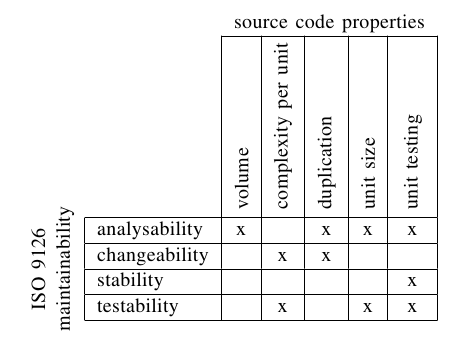
\includegraphics[width=11cm]{./imagenes/mantainability1.png}
    \caption{Cruce entre las subcaracterísticas atribuidas a la mantenibilidad del software en el estandar ISO/IEC 9126 y las propiedades a nivel de código. Cada cruce es indicado por una $x$}
    \label{fig:mantainability1}
    \textbf{Fuente:}  \cite{measuring_maintainability}
  \end{center}
\end{figure}

Así, en el presente proyecto, se ha decidido utilizar las siguientes medidas creadas por los autores:

\begin{itemize}
 
 \item \textbf{Nivel de complejidad por unidad}: El nivel de complejidad es calculado, en primera instancia, calculando la complejidad ciclomática de cada unidad del software, la cual es definida como $$cc = e – n + 2$$ donde $n$ representa a los nodos del grafo de control de flujo y $e$ el número de aristas de dicho grafo, según \cite{cyclomatic_complexity}. Luego de esto, será necesario ubicar cada unidad en un nivel de riesgo. En el siguiente cuadro se podrá observar cómo son valorados los niveles de riesgo:

\begin{figure}[!htb]
  \begin{center}
    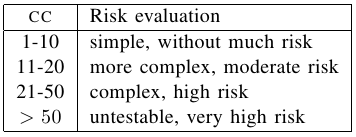
\includegraphics[width=11cm]{./imagenes/mantainability2.png}
    \caption{correspondiente al nivel de riesgo en el software presentado por la complejidad ciclomática promedio del sistema}
    \label{fig:mantainability2}
    \textbf{Fuente:}  \cite{measuring_maintainability}
  \end{center}
\end{figure}

Luego de tener dichas cuentas y, además, por cada unidad tener los LOC asociados, se ubicarán las sumas de los LOC ubicados en cada nivel de riesgo, esto es, $\sum LOC_{ij}$, donde $i$ representa el cambio en los niveles de riesgo y $j$ representa el cambio en las unidades que pertenecen a dicho nivel $i$, dentro de un nivel maximo relativo de LOC que podrían ser riesgosas al momento de mantener el software.

\begin{figure}[!htb]
  \begin{center}
    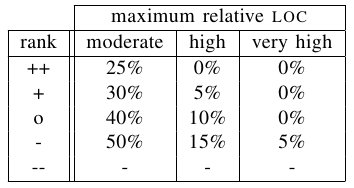
\includegraphics[width=11cm]{./imagenes/mantainability3.png}
    \caption{correspondiente al nivel máximo relativo de LOC que podrían ser riesgosas al momento de mantener el software}
    \label{fig:mantainability3}
    \textbf{Fuente:}  \cite{measuring_maintainability}
  \end{center}
\end{figure}

 \item \textbf{Duplicación}: Se utiliza una medida que, aunque básica, debido a los estandares definidos para la realización de este proyecto, se hace más precisa. La técnica, descrita en \cite{measuring_maintainability}, consiste en contar los duplicados como un bloque de 6 líneas de código exáctamente iguales en una o varias partes del software. Luego, se harán medidas relativas al dividir la cantidad de líneas de código duplicadas por la cantidad total del software, clasificando el resultado en una de las categorías mostradas en la figura \ref{fig:mantainability4}.

\begin{figure}[!htb]
  \begin{center}
    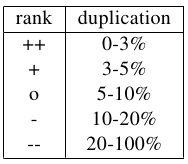
\includegraphics[width=11cm]{./imagenes/mantainability4.png}
    \caption{clasificación de duplicación de código}
    \label{fig:mantainability4}
    \textbf{Fuente:}  \cite{measuring_maintainability}
  \end{center}
\end{figure}

 \item \textbf{Volumen por unidad}: FALTANTE

\end{itemize}

En lo que concierne a la mantenibilidad de web services específicamente, se tomó de \cite{complexity_mesure} aquellas medidas que pueden ayudar a medir la mantenibilidad en un sistema SOA hecho con web services. 

En \cite{complexity_mesure}, basados en las definiciones de los documentos WSDL, los autores crean medidas de complejidad basados en la complejidad de los tipos de datos manejados, haciendo de estos un árbol formado por estructuras de datos simples y complejas. Cabe anotar que los tipos de datos complejos creados en el WSDL y puestos dentro de otro tipo de dato complejo hacen un sub-árbol, haciendo más complejo el tipo de dato que compone. La complejidad de un tipo de dato se mide por la profundidad del arbol que lo compone. Así, a continuación se explicarán las medidas utilizadas:

\begin{itemize}

 \item \textbf{Métrica de complejidad basada en mensaje}: Esta métrica busca medir la complejidad de los mensajes pasados de un servicio a otro haciendo una sumatoria de las complejidades de los tipos de datos utilizados en los mensajes, es decir: $$COM_{k} = \sum_{i=1}^{n} ci$$ donde $k$ es el k-ésimo mensaje, i es el tipo evaluado y $n$ el número de tipos que utiliza el k-ésimo mensaje.
 \item \textbf{Métrica de complejidad basada en operación}: En esta métrica se busca medir la complejidad de una operación definida en el documento WSDL. Para ello se ha de tener en cuenta que las operaciones trabajan con mensajes de salida y de entranda. Por tanto, la métrica será la media de la complejidad de todos los mensajes de salida y entrada que estén definidos en la operación, esto es: $$CBO = \frac{\sum_{i=1}^{p} COM_{i} + \sum_{j=1}^{q} COM_{o}}{m}$$ donde $p$ representa la cantidad de mensajes de entrada y $q$ representa la cantidad de mensajes de salida de la operación. Asimismo, $m$ representa la cantidad total de mensajes.

\end{itemize}

\subsection{Reusabilidad}

En \cite{computer_science}, nombra la reusabilidad como la utilización de un producto terminado para el desarrollo de otro producto, tal vez con algunos cambios sobre el original. Una de las metas de la reusabilidad, según \cite{computer_science}, es el trato de la granuralidad a un nivel en el que el software pueda ser reusado para el desarrollo de otro software. Se nombra, en \cite{computer_science}, el manejo de la granuralidad de un componente de software. En lo que a este desarrollo refiere, se deberá manejar la granuralidad de los servicios a nivel de capacidades, de complejidad de datos y a nivel de servicios, según \cite{soa_principles}.

\subsubsection{Medidas de reusabilidad}

 En \cite{soa_principles}, se propone una calificación para las medidas de reuso planeadas, estas son:

\begin{itemize}
 \item \textbf{Reusabilidad táctica}: Es la reusabilidad llevada a cabo sólo con las capacidades de los servicios que son requeridas inmediatamente.
 \item \textbf{Reusabilidad de destino}: Es la reusabilidad llevada a cabo con capacidades que serán más propensas a ser reusadas.
 \item \textbf{Reusabilidad completa}: Es la reusabilidad que equipa a un servicio con todas las características que éste puede cumplir.
\end{itemize}

Para llevar a cabo una medida del correcto reuso de los servicios, será necesario tener medidas de las capacidades de dichos servicios que son, realmente, utilizadas, tales como la cantidad de consumidores y la frecuencia con que son usadas.

\subsubsection{Blueprints y reusabilidad}

Además, en orden de hacer reusables los servicios, se debe lograr adicionar el estatus de \textit{servicio agnóstico} a la mayor cantidad de servicios posible, esto es, separando a los servicios construidos de cualquier vínculo irreparable con el negocio o con las diversas plataformas.

También, los arquitectos de información y los analistas de negocio deberán separar cuidadosamente cada servicio en cada blueprint de servicios, con motivo de agrupar los servicios por dominios de aplicación en la organización. Con esta metodología será posible una mayor separación de necesidades y, por ende, mayor desacoplamiento entre servicios.

\subsubsection{Logic Centralization: Patrón de diseño pro-reusabilidad}

Cuando se habla de reusabilidad en SOA, se habla también de un patrón de diseño llamado Logic Centralization. Este patrón es aquel que garantiza la reutilización de un mismo servicio cuando un mismo requerimiento quiera ser utilizado por un servicio consumidor. A manera de ejemplo, uno podría tener dos servicios con logica duplicada de facturación y el servicio consumidor. Esto genera un costo a largo plazo debido al re-desarrollo de capacidades ya suplidas por desarrollos anteriores. Se debe, pues, centralizar la lógica a un servicio agnóstico y utilizar este siempre que se necesite. Si este último no llegase a tener las capacidades que se requieren, será necesario entonces adicionarlas.

A su vez, el patrón de diseño Contract centralization debe ser utilizado en conjunto con Logic Centralization para poder centralizar puntos de acceso a una misma capacidad requerida por un servicio consumidor. Contract centralization requiere que los servicios consumidores se dirijan siempre al contrato del servicio como punto de acceso al mismo y nunca a otra fuente externa.

\subsubsection{Granularidad y reusabilidad}

En cuanto a granularidad, en \cite{soa_principles}, se identifica un tratamiento a esta a nivel de servicio, de capacidades de servicio y de datos. En general, el tratamiento a nivel de servicio tiende a ser hecho con grano fino debido a la filosofía de SOA, la cual lleva a la producción de servicios agnósticos primordialmente. En cuanto a las capacidades, la tendencia es a hacer versiones de grano fino y de grano grueso de cada una. En cuanto a los datos, se tiene a trabajar con grano grueso en ellos.

\subsection{QiU: Quality in Use}

En \cite{quality_in_use}, antes de hablar de la usabilidad del software, los autores nombran la existencia del concepto QiU según ISO/IEC 9126-4, el cual lo define como \textbf{La capacidad del producto de software para permitir a usuarios específicos lograr metas específicas con eficiencia, productividad, seguridad y satisfacción en contextos de uso específicos}. En QiU se define a la usabilidad como una de las cualidades que realiza la capacidad del software para ser de calidad.

\subsubsection{Usabilidad}

En \cite{quality_in_use}, se nombran algunas de las definiciones de usabilidad. Una de ellas, la definición propuesta en la ISO/IEC 9126-4, dice: \textbf{La extención por la cual un producto puede ser usado por usuarios especificos para lograr metas específicas con efectividad, eficiencia y satisfacción en un contexto específico de uso}.

A su vez, en \cite{quality_in_use}, enuncian tres acercamientos al concepto de usabilidad:

\begin{itemize}
 \item \textbf{Usabilidad de sistema}: Data del conocimiento de las metas de la organización aplicadas al sistema construido.
\item \textbf{Experiencia de usuario (UX)}: Consideración de las metas hedónicas y pragmáticas de los usuarios al momento de construir el software.
\item \textbf{Usabilidad de producto}: Soporte de UX y usabilidad del sistema al software construido.
\end{itemize}

\subsubsection{User aceptance (Aceptación de usuario)}

Se refiere, en \cite{quality_in_use}, a la acogida de un producto software por parte del cliente cuando éste cumple características específicas que \textit{atrapan} a este. Dichas características son:

\begin{itemize}
 \item \textbf{Utilidad percibida}: Esta se refiere a cuanto el software puede cumplir con las necesidades pragmáticas del usuario.
 \item \textbf{Facilidad de uso percibida}: Esta se refiere a la premisa de que el usuario busca siempre aquello que le tome menos tiempo aprender pero que, a su vez, le siga siendo útil.
\end{itemize}

\subsubsection{Experiencia de usuario (User eXperience - UX)}\label{subsec:UX}

En \cite{quality_in_use} y según la ISO 9241-210 define UX como \textbf{Las percepciones y respuestas de una persona del uso o anticipado uso de un producto, sistema o servicio}. El análisis de UX es motivado por el cómo las personas se sienten al utilizar cierto software, su nivel de satisfacción al momento de usarlo y después de ello.

Los servicios de redes sociales (SNS por sus siglas en ingles: Social Network Services) como Facebook, LinkedIn, Twitter, SportTracker o Xportia, ofrecen servicios para la gestión de la OSN de cada usuario que acceda a estas aplicaciones. Según un estudio hecho para medir la experiencia de usuario \cite{user_behavior_online} (UX por sus siglas en ingles: User eXperience) en los SNS, se encontraron 8 categorías que son críticas a la hora de diseñar una SNS y son:

\begin{enumerate}
  \item Self-expresion: Capacidad que tengan las OSN de compartir contenido relacionado a la vida real de los usuarios tal como lo pueden ser las fotos, los videos, los comentarios o las comunicaciones directas.
  \item Reciprocity: Interacción bilateral en tiempo real, es decir, interacción instantánea con uno o varios individuales en la OSN (por ejemplo, por medio de los servicios de mensajería instantánea).
  \item Learning: La información recibida por medio de la OSN debe poder ser utilizada en pro del desarrollo cognitivo del individual; debe existir información útil al individual que usa la OSN.
  \item Curiosity: El contenido de la OSN debe ser interesante para quien la utiliza.
  \item Suitability of functionality: Se refiere a cuán ``utilizable'' es una funcionalidad.
  \item Suitability of content: La calidad y exactitud de la información que en la OSN reside debe ser suficiente para el individual perteneciente a ella.
  \item Completeness of the user network: Los individuales deben querer pertenecer a la red social y buscar eficientemente a otros individuales para poder formar lazos con ellos y hacer crecer su red social.
  \item Trust and privacy: Confianza en los servicios de las OSN, así como también la capacidad que tiene el usuario de gestionar la privacidad del contenido que comparte en dicha OSN. \cite{social_experience}
\end{enumerate}

Cada uno de las categorías nombradas hace parte de los factores que impulsan la utilización de los SNS para la gestión de las OSN de las personas.

\subsubsection{Conceptos para medir QiU}

Para medir las características de QiU en el software desarrollado, se utilizaron los conceptos retratados en \cite{usability_ux}, donde los autores crearon un framework para evaluar, tanto UX como usabilidad en sistemas mobiles. Se analizaron los siguientes aspectos:

\begin{itemize}
 \item \textbf{Eficiencia}: Capacidad del producto de software para ofrecer rendimiento apropiado, visto desde la cantidad de recursos usados.
 \item \textbf{Eficacia}: Capacidad del producto de software para permitir al usuario ejecutar tareas de manera precisa, según las necesidades de éste.
 \item \textbf{Satisfacción}: Valoración de la actitud del usuario frente al software utilizado
 \item \textbf{Productividad}: Capacidad del software para permitir al usuario ser efectivo (cumplir el objetivo sin gastar cantidades grandes de recursos valiosos para él).
 \item \textbf{Learn-ability}: Puede definirse como la capacidad que tiene el software para darse a conocer al usuario.
 \item \textbf{Seguridad}: Capacidad del software de no propiciar ningún daño sobre la propiedad del usuario (su empresa, su ser, etc.).
 \item \textbf{Entendibilidad}: Capacidad que tiene el software para dar a entender al usuario para que está hecho y él pueda decidir si puede cumplir con las tareas que requiere o no.
\end{itemize}

\subsection{Seguridad}

En \cite{security_ws}, la seguridad es definida como un concepto que guía a la protección de las posesiones, ya sean tangibles o intangibles. Para hablar de seguridad, primero definen conceptos clave de seguridad. Estos últimos serán listados a continuación:

\begin{itemize}
 \item \textbf{Asset (Posesión)}: Es definido como el tangible o intangible a proteger.
 \item \textbf{Threat (Amenaza)}: Es un escenario en el cual es posible causar daño a una posesión. Esta requiere de la existencia de una vulnerabilidad para ser llevada a cabo con éxito.
 \item \textbf{Vulnerability (vulnerabilidad)}: Es una debilidad que hace una amenaza posible.
 \item \textbf{Attack (Ataque)}: Es la acción de llevar a cabo una amenaza.
\end{itemize}

Otros elementos de la seguridad, enfocada más al aspecto informático, son:

\begin{itemize}
 \item \textbf{Autenticación}: Es la presentación de los participantes de la conexión. Este concepto responde a la pregunta \textit{¿quien eres?}.
 \item \textbf{Autorización}: Es la posibilidad de un usuario (humano o no) de realizar una operación u obtener algún dato. Este concepto responde a la pregunta \textit{¿que puedes hacer?}.
 \item \textbf{Auditoría}: La revisión de los posibles vaciós presentados en temas de seguridad es manejado por la constancia de la realización de ésta actividad.
 \item \textbf{Confidencialidad}: Este concepto establece la necesidad de que la información compartida entre diferentes usuarios sea vista solo por ellos.
 \item \textbf{Integridad}: Este concepto es logrado cuando se logra proteger los datos de modificaciones indeseadas antes de que el receptor reciba un mensaje de un emisor.
 \item \textbf{Disponibilidad}: Es la seguridad de que una aplicación estará siempre disponible para usuarios legítimos.
\end{itemize}

En \cite{security_ws}, se exponen principios de seguridad en Web Services, los cuales son utilizados para definir el requerimiento no funcional seguridad. A continuación se exponen aquellos nombrados:

\begin{itemize}
 \item \textbf{Aplicar defensa en profundidad}: Uso de varios \textit{gatekeeper} (en español, portero), es decir, utilizar múltiples capas de seguridad para mantener las posesiones seguras.
 \item \textbf{Chequear en la puerta}: Utilizar la autenticación y la autorización como la primera capa de seguridad.
 \item \textbf{Compartimentar}: Limitar el rango de acción de un atacante aislando posibles vulnerabilidades.
 \item \textbf{Crear \textit{por defecto} seguros}: Este principio se refiere a la necesidad de crear usuarios por defecto que sean manejados de forma segura, esto es, limitando sus privilegios sobre recursos (datos y operaciones) que sean sensibles y, quizás, deshabilitando dicha cuenta desde un principio.
 \item \textbf{No confiar en las entradas del usuario}: Debido a que el ataque principal es hecho por medio de entradas al sistema, será necesario aplicar el principo de defensa en profundidad con dichas entradas, nunca confiando en que ellas no sean potencialmente malignas.
 \item \textbf{Establecer límites de confianza}: Este principio se refiere a la decisión de ser permisivo o no con cierto flujo de datos o entradas, con el fin de poder analizar más en profundidad que amenazas pueden presentarse en el sistema según los límites que se den a dichos datos y entradas.
 \item \textbf{Fallar siendo seguro}: Este principio dice que, cuando ocurra un error, se deben retornar mensajes amigables al usuario y que no revelen información que pueda ser usada en contra para explotar vulnerabilidades de nuestro sistema.
 \item \textbf{Reducir el área en riesgo de ataque}: Este principio se refiere al control de recursos disponibles a usuarios. Si un recurso no se usa, será mejor deshabilitarlo o eliminarlo, reduciendo así el área vulnerable.
 \item \textbf{Asegurar el enlace más débil}: Se necesita estar atento de todas las posibles partes del sistema que puedan tener más vulnerabilidades y, por lo tanto, ser utilizadas para atacar el sistema.
 \item \textbf{Usar menos privilegios}: Al restringir privilegios a usuarios, es menos probable que un atacante pueda explotar las posibles vulnerabilidades de un sistema, no podrá utilizar ciertos recursos para atacarlo.
\end{itemize}